\chapter{Posterior distributions of regression model parameters under Maruyama's Beta-Prime prior}

\section{Introduction}

In this chapter, we consider
a linear model with $g$-priors used for model selection, as in \citep{Maruyama2011}. 
In most cases, we derive exact expressions for the posterior distributions of the regression parameters of
this model. Where this is analytically intractable, we derive exact expressions for the expectation and
covariance of the regression parameters, and develop a Laplace approximation to the posterior distribution
of the regression parameters.

% Structured Variational Bayes for model selection, Wand and Ormerod Variational Bayes for Elaborate 
% Distributions (\citep{Wand2011})

% Application

% VB theory

% Our main contribution
In this paper, we develop Variational Bayes approximations to model selection of linear models using Zellner's
g prior as in \citep{Liang2008}.

% By searching of the model space as one covariate changes between each sub-model and  using rank-1 updates on
% $(\mX^\top \mX)^{-1}$, we are able to exhaustively search the model space in $\BigO(2^p np^2)$ rather than
% $\BigO(2^p np^3)$.

% This article is organised as follows. In Section \ref{sec:model_selection}, we review previous Bayesian
% approaches to model selection. 
In Section \ref{sec:methodology} we develop our approach. In Section
\ref{sec:num_exp} we perform a series of numerical experiments to show the accuracy of our approach. Finally,
in Section \ref{sec:conclusion}, we provide a Conclusion and Discussion.

\section{Methodology}
\label{sec:methodology}

\subsection{Notation}

% Definitions

Let $n > 0$ be the number of observations and $p > 0$ be the number of covariates. Let $\vy \in \R^n$ be the
vector of responses, $\vtheta \in \R^p$ be the vector of parameters and $\mX \in \R^{n \times p}$ be the
matrix of covariates. Let $p(\vtheta)$ be the prior distribution of $\vtheta$, $p(\vy, \vtheta)$ be the full
probability distribution of $\vy$, $p(\vtheta | \vy)$ the posterior distribution and $q(\vtheta)$ be the
approximating probability distribution. 

\subsection{Model}
\label{sec:model}

Zellner constructed the $g$-prior family of priors for a Gaussian regression model using a particular form of
conjugate Normal-Gamma model, where the prior covariance matrix of $\vbeta$ is taken to be a multiple of the
Fisher information  matrix by the parameter $g$ \citep{Zellner1986}. This could be thought of as regularisation
in the principle components of the estimated covariance matrix. This places the most prior mass for $\vbeta$
on the section of the parameter space where the data is least informative.

We consider a normal linear model on $\vy$ with conjugate normal prior on $\vbeta$, and covariance $g \sigma^2
(\mX^\top \mX)^{-1}$ where the prior on $g$ is Zellner's g-prior on the covariance matrices, 
We consider a normal linear model with a $g$-prior on the regression co-efficients $\vbeta$.
This introduces a hyperparameter $g$ which controls the shrinkage of the regressions co-efficients.
The prior on $g$ can be carefully chosen so that the other parameters in the model can be integrated out
analytically, yielding tractable marginal and posterior distributions for $g$, as shown by \citep{Liang2008}.
Several priors on $g$ have been considered in the literature, including the hyper-$g$ and hyper-$g/n$ priors
\cite{Liang2008}, Bayarri's robust prior \cite{Bayarri2012} and the Beta-Prime prior introduced by
\citep{Maruyama2011}. We choose the popular Beta-Prime prior, as it is numerically well-behaved. 
We choose $a$  and $b$ to be $-3/4$ and $(n - p)/2 - a - 2$ respectively, following \citep{Maruyama2011}.

\section{The base model}
\label{sec:model}

Suppose $\vy = (y_1,\ldots,y_n)^T$ is a response vector of length $n$, $\mX$ is an $n$ by $p$ matrix 
of covariates. We consider the linear model for predicting $\vy$ with predicturs $\mX$ via
\begin{equation}
\label{eq:linearModel}
\vy | \alpha, \vbeta, \sigma^2 \sim N(\vone_n\alpha + \mX \vbeta, \sigma^2 \mI_n),
\end{equation} 


\noindent where $\alpha$ is the model intercept, $\vbeta$ is a coefficient vector of length $p$, 
$\sigma^2$ is the residual variance, and $\mI_n$ is the $n \times n$ identity matrix. 
Without loss of generality, to simplify later calculations, we will transform $\vy$ and $\mX$ 
so that $\vy$ and the columns of $\mX$ are standardized so that $\overline{y} = 0$, 
$\|\vy\|^2 = \vy^T\vy = n$, $\mX_j^T\vone = 0$,  and $\|\mX_j\|^2 = n$ where $\mX_j$ is the $j$th  column of $\mX$. 

Suppose that we wish to perform Bayesian model selection, model averaging or hypothesis 
testing. Let $\vgamma \in \{0, 1\}^p$ be a binary vector of indicators
for the inclusion of the $p$th column of $\mX$ in the model where $\mX_\vgamma$ 
denotes the design matrix formed by including only the columns of $\mX$ with 
$\gamma_j = 1$. We will adopt the following prior structure
\begin{equation}
\label{eq:priorStructure}
\begin{array}{c}
\ds p(\alpha) \propto 1,  
\qquad 
\ds p(\sigma^2) \propto (\sigma^2)^{-1} I(\sigma^2 > 0),                      
\\ [2ex]
\vbeta_\vgamma | \sigma^2, g, \vgamma \sim \N_p(\vzero, g \sigma^2 (\mX_\vgamma^T \mX_\vgamma)^{-1}),
\quad \text{ and }  \quad 
p(\vbeta_{-\vgamma}|\vgamma) = \prod_{j=1}^p \delta(\beta_j;0)^{1-\gamma_j},
\end{array}
\end{equation} 

\noindent where $\delta(x;a)$ is the Dirac delta function with location $a$. 
For the time being we will defer specification of $p(g)$ and $p(\vgamma)$.
We will now justify each element of our chosen prior structure.

The priors on $\alpha$ and $\sigma^2$ are improper Jeffreys priors and have been formally justified 
in \cite{Berger2012}. In the context Bayesian model selection, model averaging or hypothesis 
testing $\alpha$ and $\sigma^2$ appear in all models 
so that when comparing models the proportionality constants in the corresponding
Bayes factors cancel.

The prior on $\vbeta_\vgamma$ is Zellner's $g$-prior \citep[see for example,][]{Zellner1986} with prior 
hyperparameter $g$. This family of priors for Gaussian regression model where the prior covariance 
matrix of $\vbeta_\vgamma$ is taken to be a multiple of $g$ with the Fisher information matrix for $\vbeta$. 
This places the most prior mass for $\vbeta_\vgamma$ on the section of the parameter space where the data is 
least informative, and makes the marginal likelihood of the model scale-invariant. Furthermore, this 
choice of prior removes a log-determinant of $\mX_\vgamma^T\mX_\vgamma$ term from the expression for the marginal 
likelihood, which is an additional computational burden to calculate.

\section{Exact posterior distributions in terms of special functions}
\label{sec:Exact}
 
In this section we derive the exact expressions for most Bayesian inferential quantities
of interest based on the model presented in Section 2. An exception is
the exact expression for the posterior density for $\vbeta|\vy$ for this quantity we
instead derive the first and second moments.


First, we use the fact that $p(\sigma^2|\vy) = \int_0^\infty p(\sigma^2|\vy,u) p(u|\vy)dg$ so that the density
$\sigma^2|\vy$ may be expressed as
$$
\begin{array}{rl}
\ds p(\sigma^2|\vy) 
%& \ds = 
%\left[ \frac{\left(\tfrac{n}{2}\right)^c}{\Gamma(c)} (\sigma^2)^{-(c+1)} \exp\left\{ - \frac{n}{2\sigma^2} \right\} \right] 
%\left[ \frac{(1 -  R^2)^{b+1} }{\mbox{Beta}(d + 1,b+1)} %\right] \int_0^\infty 
% g^{b} (1 + g)^{-c}  \exp\left(   \frac{g}{1+g} \frac{nR^2}{2\sigma^2} \right) dg.
%\\
& \ds = 
\left[ \frac{\left(\tfrac{n}{2}\right)^c}{\Gamma(c)} (\sigma^2)^{-(c+1)} \exp\left\{ - \frac{n}{2\sigma^2} \right\} \right] 
\left[ \frac{(\widehat{\sigma}^2)^{b+1} }{\mbox{Beta}(d + 1,b+1)} \right]
\int_0^1
u^{b} (1 - u)^d  \exp\left(  \frac{nR^2}{2\sigma^2} u \right) du.
\end{array}
$$

%\noindent \joc{
%$$
%u = \frac{g}{1+g},
%\quad 
%g = \frac{u}{1-u},
%\quad 
%1 - u = \frac{1}{(1 + g)},
%\quad 
%(1 - u)^{-1} = (1 + g),
%\quad \mbox{and}\quad 
%\frac{du}{dg} = \frac{1}{1+g} - \frac{g}{(1 +g)^2} 
%= \frac{1}{(1+g)^2} = (1 - u)^2.
%$$
%
%\noindent Using the change of variables $u = g/(1 + g)$ the integral
%above is  
%$$
%\ds \int_0^1 u^{b} (1 - u)^d  \exp\left(  %\frac{nR^2}{2\sigma^2} u \right) du
%= \mbox{Beta}(d+1,b+1) {}_1 F_1\left(b + 1; c; %\frac{nR^2}{2\sigma^2} \right)
%$$
%
%$$
%	\int_{0}^u x^{\nu - 1} (u - x)^{\mu - 1}  e^{\beta x} dx = \mbox{Beta}(\nu,\mu) {}_1 F_1(\nu;\mu+\nu;\beta u) \quad   \mbox{(assuming $\mbox{Re}(\mu)>0$ and $\mbox{Re}(\nu)>0$).}
%$$
%\noindent with $u = 1$, $\nu = b + 1$, $\mu = a + p/2 + 1 >0$, and $\beta = nR^2/(2\sigma^2)$.
%}

\noindent 
Utilising Equation 3.383(i) of \cite{Gradshteyn2007} (see Appendix A) we obtain  
$$
%\begin{array}{rl}
\ds p(\sigma^2|\vy) 
%& 
\ds = 
\frac{\left(\tfrac{n}{2}\right)^c (\widehat{\sigma}^2)^{b+1}}{\Gamma(c)} (\sigma^2)^{-(c+1)} \exp\left(  - \frac{n}{2\sigma^2} \right)
{}_1 F_1\left(b + 1; c; \frac{nR^2}{2\sigma^2} \right),
%\end{array}
$$

\noindent where 
${}_1 F_1(\alpha;\gamma;z)$ 
is the confluent hypergeometric function (also called
Kummer's function of the first kind).
To the best of our knowledge, this is a new positive valued continuous distribution.
An alternative representation using the identity ${}_1F_1(a;b;z) = e^z {}_1F_1(b-a;b;-z)$ results in
$$
%\begin{array}{rl}
\ds p(\sigma^2|\vy) 
%& 
\ds = 
\frac{\left(\tfrac{n}{2}\right)^c (\widehat{\sigma}^2)^{b+1}}{\Gamma(c)} (\sigma^2)^{-(c+1)} \exp\left(  - \frac{n \widehat{\sigma}^2}{2\sigma^2} \right)
{}_1 F_1\left( d + 1; c; -\frac{nR^2}{2\sigma^2} \right),
%\end{array}
$$

\noindent which is much more amenable to numerical evaluation. 
 
 
Next we have
$p(\alpha|\vy) = \int_0^\infty p(\alpha|\vy,\sigma^2)p(\sigma^2|\vy) d\sigma^2$.
% where $\alpha|\vy,\sigma^2 \sim N(0,\sigma^2/n)$. 
After we apply the change of variables $\sigma^2 = 1/\tau$
we obtain
$$
\begin{array}{rl}
\ds p(\alpha|\vy) 
%& \ds =
%\joc{ \frac{\left(\tfrac{n}{2}\right)^c (1 -  R^2)^{b+1}  }{\Gamma(c)\sqrt{2\pi/n}}
%\int_0^\infty 
%(\sigma^2)^{-1/2} \exp\left( -\frac{n\alpha^2}{2\sigma^2} \right) 
%(\sigma^2)^{-(c + 1)}\exp\left( -\frac{n}{2\sigma^2}  \right)  {}_1 F_1\left( b + 1; c; %\frac{nR^2}{2\sigma^2} \right)  d\sigma^2
%}
%\\ [2ex]
%& \ds =  \frac{\left(\tfrac{n}{2}\right)^c (1 -  R^2)^{b+1}  }{\Gamma(c)\sqrt{2\pi/n}} 
%\times 
%\int_0^\infty 
%(\sigma^2)^{-c -3/2} \exp\left( -\frac{n(1+\alpha^2)}{2\sigma^2} \right)   {}_1 F_1\left( b + %1; c; \frac{nR^2}{2\sigma^2} \right) d\sigma^2
%\\
& \ds = \frac{\left(\tfrac{n}{2}\right)^c (1 -  R^2)^{b+1}  }{\Gamma(c)\sqrt{2\pi/n}} 
\times 
\int_0^\infty 
\tau^{c - 1/2} \exp\left( -\frac{n(1+\alpha^2)}{2} \tau \right)   {}_1 F_1\left( b + 1; c; \frac{nR^2}{2} \tau \right) d \tau.
\end{array}
$$


%$$
%\begin{array}{rll}
%\ds \int_0^\infty e^{-st} t^{b-1} {}_1F_1(a,c,kt) dt
%& \ds = \Gamma(b)s^{-b} F(a,b,c,k s^{-1}) 
%& \mbox{(if $|s| > |k|$)}
%\\
%& \ds = \Gamma(b)(s - k)^{-b} F\left(c - a, b; c; \frac{k}{k - s} %\right)
%& \mbox{(if $|s - k| > |k|$)}
%\end{array} 
%$$

%\noindent assuming that $\mbox{Re}(b)>0$, $\mbox{Re}(s) > %\max(0,\mbox{Re}(k))$. 
%In the above case
%$$
%b \leftrightarrow c + 1/2, \quad 
%s \leftrightarrow \frac{n(1+\alpha^2)}{2} , \quad
%a \leftrightarrow b + 1, \quad 
%c \leftrightarrow c, \quad \mbox{and} \quad
%k \leftrightarrow  \frac{nR^2}{2}.
%$$


%\noindent where the second line above follows from the 
%change of variables $\sigma^2 = 1/\tau$.

%\joc{
%\noindent Equation 7.621 (4) of \cite{Gradshteyn2007} 
%(the second line corrected from EH I, 269(5))
%is

%
%\noindent The first holds since
%$$
%|s| = \frac{n(1+\alpha^2)}{2}  > |k| = \frac{nR^2}{2} \qquad %\mbox{(since $R^2 \in [0,1]$ and $\alpha^2\ge 0$)},
%$$
%
%\noindent Checking the other conditions
%$$
%b \leftrightarrow c + 1/2 = (n-1)/2 + 1/2 = n/2 > 0.
%$$
%}

\noindent 
Utilizing  Equation 7.621 (4) of \cite{Gradshteyn2007} we obtain
\begin{equation}\label{eq:alphaGivenY}
\begin{array}{rl}
\ds p(\alpha|\vy) 
& \ds = \frac{ \Gamma\left( c + \tfrac{1}{2} \right) (1 -  R^2)^{b+1}  }{ \Gamma(c)\sqrt{\pi}} 
\left( 1+\alpha^2 \right)^{-n/2} {}_2F_1\left( b+1, c + \frac{1}{2}; c; \frac{R^2}{1+\alpha^2}  \right),
\end{array}
\end{equation}

\noindent where ${}_2F_1$ is the Gaussian hypergeometric function.

The first three arguments of the ${}_2F_1$ function in (\ref{eq:alphaGivenY}) are $O(n)$. This makes 
numerical evaluation of (\ref{eq:alphaGivenY}) difficult in general. In order to handle this difficulty
we will first use the Euler transform
Euler's identity 
${}_{2}F_{1}(a,b;c;z)=(1-z)^{c-a-b}\,{}_{2}F_{1}(c-a,c-b;c;z)$ leading to
\begin{equation}\label{eq:alphaGivenY_2}
	\begin{array}{rl}
		\ds p(\alpha|\vy) 
		& \ds = \frac{ \Gamma\left( c + \tfrac{1}{2} \right)   }{ \Gamma(c)\sqrt{\pi}} 
		\frac{(1 -  R^2)^{b+1}}{(  \alpha^2 + 1 - R^2 )^{b+3/2}}
		\left( 1+\alpha^2 \right)^{ - (d+1) }   
		
		 {}_2F_1\left( d + 1,  - \frac{1}{2}; c; \frac{R^2}{1+\alpha^2}  \right),
	\end{array}
\end{equation}

\noindent which is again more numerically stable to evaluate
when $n$ is large.
 
Unfortunately, we have not been able to find a closed form expression
for $\vbeta|\vy$ in terms of known special functions. However,
it is possible, for fixed $\vbeta$ to integrate $\int p(\vbeta|\vy,u)p(u|\vy)du$
using  (\ref{eq:uGiveY})  and (\ref{eq:betaGivenYandU})
%, i.e.,
%$$
%\begin{array}{rl}
%\ds p(\vbeta|\vy)
%& \ds =  \frac{(1 -  R^2)^{b+1} \Gamma\left( \tfrac{n+p-1}{2}\right)
%	|\mX^T\mX|^{1/2} n^{(n+p-1)/2} }{\mbox{Beta}(b + 1,d+1) \Gamma\left( \tfrac{n-1}{2} \right) n^{p/2}\pi^{p/2}  } \\
%& \ds \quad \times \int_0^1
%u^{b - p/2 + (n+p-1)/2}  (1 - u)^d (  1 -  uR^2 )^{-(b + d + 2)-p/2 + (n+p-1)/2}  
%\left[ n u \left( 1 - u R^2\right) + (\vbeta - u\widehat{\vbeta})^T
%\mX^T\mX
%(\vbeta - u\widehat{\vbeta}) \right]^{-(n+p-1)/2} du
%\end{array}
%$$ 
via univariate numerical integration methods.
Instead we will concentrate on deriving the first and second moments of $\vbeta|\vy$.


In order to calculate the first and second posterior moments for $\vbeta$
we use the laws of total expectation and variance respectively, i.e.,
%$\bE(\vbeta|\vy) = \bE_{g|\vy}\left[ \vbeta|\vy,g \right]$, and
%$\mbox{Cov}(\vbeta|\vy)  = \bE_{g|\vy}\left[
%\mbox{Cov}(\vbeta|\vy,g)
%\right] + \mbox{Cov}_{g|\vy}\left[
%\bE(\vbeta|\vy,g)
%\right]$ 
%or equivalently 
$\bE(\vbeta|\vy) = \bE\left[ \bE(\vbeta|\vy,u) |\vy \right]$, and
$\mbox{Cov}(\vbeta|\vy)  = \bE\left[
\mbox{Cov}(\vbeta|\vy,g)|\vy
\right] + \mbox{Cov}\left[
\bE(\vbeta|\vy,u)|\vy
\right]$ 
to obtain
$$
\begin{array}{rll}
\ds \bE(\vbeta|\vy) 
& \ds = M_1 \widehat{\vbeta}
\\ %[1ex]
\ds \mbox{Cov}(\vbeta|\vy) 
%& \ds = \bE_{u|\vy}\left[ \frac{n - 1}{n - 3}
%\left(\frac{n}{n-1}\right) u \left( 1 - u R^2\right) %(\mX^T\mX)^{-1}
%\right] + \mbox{Cov}_{u|\vy}\left[
%u \widehat{\vbeta} \right] 
%\\ [2ex]
& \ds = \tfrac{n}{n - 3} 
\left( M_1 - M_2 R^2\right) (\mX^T\mX)^{-1}
+ (M_2 - M_1^2) \widehat{\vbeta}  \widehat{\vbeta}^T
\end{array}
$$

\noindent where
$M_1 
%= \bE\left[  \left. \frac{g}{1 + g}  \right| \vy\right] 
= \bE(u|\vy)$
and
%\qquad \mbox{and} \qquad 
$M_2 
%= \bE\left[ \left. \left(\frac{g}{1 + g}\right)^2   \right| \vy \right]
= \bE(u^2|\vy)$.


Using the normalizing constant for the GH distribution,
Euler's identity and properties of the Beta function we obtain
\begin{equation}\label{eq:M1}
\begin{array}{rl}
\ds M_1 
%& \ds \joc{ = \frac{\mbox{Beta}(b + 2,d+1)}{\mbox{Beta}(b + 1,d + 1)} (1 -  R^2)^{b+1} {}_2F_1(b+d+2,b+2;b+d+3; R^2)
%}
%\\
%& \ds \joc{= 
%	\frac{\mbox{Beta}(d+1, b+2)}{\mbox{Beta}(d + 1, b + 1)} 
%	(1 - R^2)^{b+1}
%	{}_2 F_1 (c, b + 2; c + 1; R^2)
%}
%\\ [2ex]
%& \ds  \joc{=    \frac{\mbox{Beta}(d+1, b+2)}{\mbox{Beta}(d + %1, b + 1)} 
%	(1 - R^2)^{b+1}
%	\times (1 - R^2)^{c + 1 - c - (b+2)}
%	{}_2 F_1 (c + 1 - c, c + 1 - (b + 2); c + 1; R^2)        
%}
%\\ [2ex]
%& \ds  \joc{=    
%	\frac{\Gamma(b+2)}{\Gamma(c + 1)}
%	\frac{\Gamma(c)}{\Gamma(b+1)}
%	{}_2 F_1 (d + 1, 1; c + 1; R^2)        
%}
%\\ [2ex]
& \ds  =    
\frac{b + 1}{c}
{}_2 F_1 (d + 1, 1; c + 1; R^2)    
\end{array} 
\end{equation}

%\noindent Note that the same results can be obtained using 
%\cite{Gradshteyn2007} Equation 3.197 (5).

\noindent 
and,
\begin{equation}\label{eq:M2}
\begin{array}{rl}
\ds M_2
%& \ds \joc{ = \frac{(1 - R^2)^{b+1}}{\mbox{Beta}(d + 1, b + 1)} 
%	\int_0^\infty g^{b+2} (1 + g)^{-2} [1 + g (1 - R^2)]^{-c} dg 
%}
%\\ [2ex]
%& \ds \joc{= 
%\frac{\mbox{Beta}(d + 1, b+3) }{\mbox{Beta}(d + 1, b + 1)} 
%(1 - R^2)^{b+1} {}_2 F_1 (c, b+3; c + 2; R^2)
%}
%\\
%& \ds \joc{= 
%\frac{\Gamma(b+3)}{\Gamma(c + 2)}
%\frac{\Gamma(c)}{\Gamma(b+1)}
%{}_2 F_1(d+1, 2; c+ 2; R^2)    
%}
%\\
& \ds =
\frac{(b+1)(b+2)}{c(c+1)}    {}_2 F_1(d+1, 2; c+ 2; R^2).    
\end{array} 
\end{equation}

\section{Fully Bayesian inference}

In this section, we derive the expressions required for exact Bayesian inference for the model presented in
Section \ref{sec:model}. Throughout the rest of this chapter, we will assume without loss of
generality that $\vy^\top\vone = 0$ and that $\|\vy\|^2 = n$.

\subsection{Derivation of the marginal likelihood}

%\medskip 
%\noindent {\bf Result 4:}
%$\begin{array}{rl}
%\ds p(\vy|\sigma^2,g)  = \exp\left\{
%-\tfrac{n}{2}\log(2\pi\sigma^2) 
%- \tfrac{p}{2}\log(1+g)
%- \sigma^{-2} \tfrac{n}{2}\left( 
%1 -
% \tfrac{g}{1+g} R^2  \right)
%\right\}
%\end{array}$
 
\noindent First we derive the conditional likelihood of $\vy$ given $\sigma^2$ and $g$ via
$$
\begin{array}{rl}
	\ds p(\vy|\sigma^2,g) 
	  & \ds = \int \exp\left\{ 
	-\tfrac{n}{2}\log(2\pi\sigma^2) - \tfrac{1}{2\sigma^2}\|\vy - \mX\vbeta\|^2
	-\tfrac{p}{2}\log(2\pi g\sigma^2) + \tfrac{1}{2}\log|\mX^T\mX| - \tfrac{1}{2g\sigma^2}\vbeta^T\mX^T\mX\vbeta
	\right\} d\vbeta
	\\ [2ex]
	  & \ds = \quad \exp\left\{      
	-\tfrac{n}{2}\log(2\pi\sigma^2) - \tfrac{1}{2\sigma^2}\|\vy\|^2 -\tfrac{p}{2}\log(2\pi g\sigma^2) + \tfrac{1}{2}\log|\mX^T\mX| \right\}
	\\
	  & \ds \quad \times \int 
	\exp\left\{ - \tfrac{1}{2}\vbeta^T \left[ \sigma^{-2}(1+g^{-1})\mX^T\mX \right]\vbeta + \sigma^{-2}\vbeta^T\mX^T\vy
	\right\} d\vbeta \\ [2ex]
	  & \ds = \quad \exp\left\{      
	-\tfrac{n}{2}\log(2\pi\sigma^2) - \tfrac{1}{2\sigma^2}\|\vy\|^2 -\tfrac{p}{2}\log(2\pi g\sigma^2) + \tfrac{1}{2}\log|\mX^T\mX| \right\}
	\\
	  & \ds \quad \times      
	|2\pi \left[ \sigma^{-2}(1+g^{-1})\mX^T\mX \right]^{-1}|^{1/2}\exp\left\{  \tfrac{1}{2\sigma^2}  \vy^T\mX\left[ (1+g^{-1})\mX^T\mX \right]^{-1}\mX^T\vy
	\right\}
	\\ [2ex]
	  & \ds = \quad \exp\left\{      
	-\tfrac{n}{2}\log(2\pi\sigma^2) 
	- \tfrac{1}{2\sigma^2}\|\vy\|^2 
	-\tfrac{p}{2}\log(2\pi g\sigma^2) 
	+ \tfrac{1}{2}\log|\mX^T\mX| \right\}
	\\
	  & \ds \quad \times      
	\exp\left\{ 
	\tfrac{p}{2}\log(2\pi) 
	+ \tfrac{p}{2}\log(\sigma^2)
	- \tfrac{p}{2}\log(1+g^{-1})
	- \tfrac{1}{2}\log|\mX^T\mX| 
	+ \tfrac{1}{2\sigma^2}  \vy^T\mX\left[ (1+g^{-1})\mX^T\mX \right]^{-1}\mX^T\vy
	\right\}
	\\ [2ex]
	  & \ds = \exp\left\{      
	-\tfrac{n}{2}\log(2\pi\sigma^2) 
	- \tfrac{p}{2}\log(1+g)
	- \tfrac{n}{2\sigma^2} 
	+ \tfrac{g}{2\sigma^2(1+g)} n R^2
	\right\}
\end{array}
$$

\noindent where the third and last lines follow from
Equation \ref{res:01} and Equation \ref{res:02} respectively.
We also make use of the fact that $\|\vy\|^2 = n$ and the property of determinants that $|c\mA| = c^d|\mA|$ and $|\mA^{-1}| = |\mA|^{-1}$ when $\mA \in\bR^{d\times d}$.

%\medskip 
%\noindent {\bf Result 4:}
%$\ds p(\vy|g) = \frac{\Gamma(n/2)}{\pi^{n/2} \|\vy\|^n} (1 + g)^{(n-p)/2} \left[  1 + g(1 -  R^2) \right] ^{-n/2}$.

Next, we obtain the likelihood of $\vy$ conditional on $g$ by integrating out $\sigma^2$ via
$$
\begin{array}{rl}
	\ds p(\vy|g) 
	  & \ds = \exp\left\{
	- \tfrac{n}{2}\log(2\pi) - \tfrac{p}{2}\log(1+g) 
	- \tfrac{1}{2\sigma^2}n
	\right\}
	\\ [1ex]
	  & \ds \quad \times                                                                                 
	\int_0^\infty (\sigma^2)^{-(n/2 + 1)}
	\exp\left\{
	- \sigma^{-2} \left[ \tfrac{n}{2} - \tfrac{g}{2(1+g)} nR^2 \right] 
	\right\} d\sigma^2
	\\ [2ex]
	  & \ds = \exp\left\{                                                                                 
	- \tfrac{n}{2}\log(2\pi) - \tfrac{p}{2}\log(1+g)
	\right\}
	\times 
	\frac{\Gamma(n/2)}{\ds \left[ \tfrac{1}{2}\|\vy\|^2 - \tfrac{g}{2(1+g)}nR^2 \right] ^{n/2}}
	\\ [2ex]
	%    & \ds = \frac{\Gamma(n/2)}{(n\pi)^{n/2}} (1 + g)^{-p/2} \left[  1 - \frac{g}{(1+g)}  R^2 \right] ^{-n/2}
	%    \\ [2ex]
	  & \ds = \frac{\Gamma(n/2)}{(n\pi)^{n/2}} (1 + g)^{(n-p)/2} \left[  1 + g(1 -  R^2) \right] ^{-n/2}. 
\end{array}
$$

\noindent Finally, we derive the marginal likelihood of $\vy$ by integrating out $g$. Using $b= (n-p)/2 - 2 - a$ we have
$$
\begin{array}{rl}
	\ds p(\vy) 
	  & \ds = \int_0^\infty                                         
	\frac{g^{b}(1 + g)^{-a-b-2}}{\mbox{Beta}(a+1,b+1)}
	\frac{\Gamma(n/2)}{(n\pi)^{n/2}} (1 + g)^{(n-p)/2} \left[  1 + g(1 -  R^2) \right]^{-n/2}
	dg
	\\ [2ex]
	  & \ds = \frac{\Gamma(n/2)}{(n\pi)^{n/2} \mbox{Beta}(a+1,b+1)} 
	\int_0^\infty g^{b} \left[  1 + g(1 -  R^2) \right]^{-n/2}
	\\ [2ex]
	  & \ds = \frac{\Gamma(n/2) }{(n\pi)^{n/2}}                     
	\frac{\mbox{Beta}( p/2 + a + 1,b+1)}{\mbox{Beta}(a+1,b+1)}
	(1 -  R^2)^{-(b+1)}.
	\\ [2ex]
	  & \ds                                                         
	= \frac{\Gamma( p/2 + a + 1)}{(n\pi)^{n/2}} 
	\frac{\Gamma((n-p)/2)}{\Gamma(a+1)} (1 -  R^2)^{-((n-p)/2 - a - 1)} \\
\end{array}
$$

\subsection{Posterior distributions of the parameters}
We now derive the expressions for the posterior distributions of each of the parameters. Using Equation
\ref{res:03} and Equation \ref{res:04} we have
\begin{equation}
\begin{array}{rl}\label{res:06}
	p(g|\vy) & = \frac{(1 -  R^2)^{b+1} g^{b} \left[  1 + g(1 -  R^2) \right]^{-n/2}}{\mbox{Beta}(p/2 + a + 1,b+1)} \text{ and } \\
	\ds \frac{\mbox{Beta}(p/2 + a + 1,b)}{\mbox{Beta}(p/2 + a + 1,b+1)}
	  & \ds = \frac{\Gamma(p/2 + a + 1)\Gamma(b)}{\Gamma(p/2 + a + 1 + b)} 
	\frac{\Gamma(p/2 + a + 1 + b + 1)}{\Gamma(p/2 + a + 1)\Gamma(b+1)}
	\\
	  & \ds = \frac{\Gamma(b)}{\Gamma(p/2 + a + 1 + b)}                    
	\frac{\Gamma(p/2 + a + 1 + b + 1)}{\Gamma(b+1)}
	\\
	  & \ds = \frac{p/2 + a + 1 + b}{b}                                    
	\\
	  & \ds = 1 + \frac{p/2 + a + 1}{b}.                                   
\end{array}
\end{equation}
\noindent Using the change of variables $h=g/(1+g)$ we have
\begin{equation}
	p(h|\vy) = \frac{(1 -  R^2)^{b+1}}{\mbox{Beta}(p/2 + a + 1,b+1)} h^{b}(1 - h)^{2-b+n/2}  (1  - h R^2)^{-n/2}.
\end{equation}
 

\noindent The full conditional for $\vbeta$ is given by
\begin{equation}
	\begin{array}{rl}
		\vbeta|\vy,\sigma^2,g \sim \N\left[                  
		\tfrac{g}{1+g}\widehat{\vbeta}_{\mbox{\tiny LS}},    
		\tfrac{g}{1+g} \sigma^2 \left( \mX^T\mX \right)^{-1} 
		\right]                                              
	\end{array} 
\end{equation}
\noindent where $\widehat{\vbeta}_{\mbox{\tiny LS}} = \left( \mX^T\mX \right)^{-1}\mX^T\vy$.

The full conditional for $\sigma^2$ obtained by integrating out $\vbeta$ is
\begin{equation}
	\sigma^2|\vy,g \sim \mbox{IG}\left[\tfrac{n}{2},\tfrac{n}{2}\left( 
		1 -
	\tfrac{g}{1+g} R^2\right) \right].
\end{equation}

The density for $p(\sigma^2|\vy)$ is obtained by evaluating the integral
$$
\begin{array}{rl}
	\ds p(\sigma^2|\vy) 
	  & \ds = \int_0^\infty p(\sigma^2|\vy,g) p(g|\vy) dg                                                                                                                                  
	    
	\\ [2ex]
	    
	  & \ds = \int_0^\infty                                                                                                                                                                
	\left[ \frac{\left[\tfrac{n}{2}\left( 
	1 -
	\tfrac{g}{1+g} R^2\right) \right]^{n/2}}{\Gamma(n/2)} (\sigma^2)^{-(n/2 + 1)} \exp\left\{ - \sigma^{-2} \tfrac{n}{2}\left( 
	1 -
	\tfrac{g}{1+g} R^2\right) \right\} \right]
	\\ [2ex]
	  & \ds \quad \times \left[                                                                                                                                                           
	\frac{(1 -  R^2)^{b+1} g^{b} \left[  1 + g(1 -  R^2) \right]^{-n/2}}{\mbox{Beta}(p/2 + a + 1,b+1)}
	\right] dg
	    
	\\ [2ex]
	    
	    
	    
	  & \ds = \frac{(1 -  R^2)^{b+1} \left( \frac{n}{2}\right)^{n/2}(\sigma^2)^{-(n/2 + 1)}\exp\left\{ -  \tfrac{n}{2\sigma^2} \right\}}{\Gamma(n/2)\mbox{Beta}(p/2 + a + 1,b+1)}          
	\\ [2ex]
	  & \ds \quad \times \int_0^\infty                                                                                                                                                     
	\left( 
	1 -
	\tfrac{g}{1+g} R^2\right)^{n/2} g^{b} \left[  1 + g(1 -  R^2) \right]^{-n/2}
	\exp\left\{ 
	\frac{g}{1+g} \frac{nR^2}{2\sigma^2} \right\} dg
	
	\\ [2ex]
	
	  & \ds = \frac{(1 -  R^2)^{b+1} \left( \frac{n}{2}\right)^{n/2}(\sigma^2)^{-(n/2 + 1)}\exp\left\{ -  \tfrac{n}{2\sigma^2} \right\}}{\Gamma(n/2)\mbox{Beta}(p/2 + a + 1,b+1)}          
	\\ [2ex]
	  & \ds \quad \times \int_0^1                                                                                                                                                          
	\left( 
	1 -
	h R^2\right)^{n/2} \left( \frac{h}{1 - h}\right)^{b} \left[  1 + \frac{h}{1 - h}(1 -  R^2) \right]^{-n/2}
	\exp\left\{ 
	h \frac{nR^2}{2\sigma^2} \right\}\frac{1}{(1-h)^2} dh
	    
	\\ [2ex]
		
	  & \ds = \frac{ (1 -  R^2)^{b+1}\left( \frac{n}{2}\right)^{n/2}(\sigma^2)^{-(n/2 + 1)}\exp\left\{ -  \tfrac{n}{2\sigma^2} \right\}}{\Gamma(n/2)\mbox{Beta}(p/2 + a + 1,b+1)} \int_0^1 
	h^{b}(1-h)^{a+p/2} 
	\exp\left\{ 
	h \frac{nR^2}{2\sigma^2} \right\}  dh    
\end{array}
$$

% \mgc{How is this used?}
% $$
% -b-2+n/2 = p/2 + a  
% $$

\noindent using the substitution $h = g/(1 + g)$, to transform the integral to be over the interval $[0, 1]$
and into a form where we are able to use
% $g = \frac{h}{1-h}$,
% $1 - h = \frac{1}{(1 + g)}$,
% and
% $\frac{dh}{dg} = \frac{1}{1+g} - \frac{g}{(1 +g)^2} = \frac{1}{(1+g)^2} = (1 - h)^2$.
Equation 3.383(i) of \citep{Gradshteyn1988},
$$
\int_{0}^u x^{\nu - 1} (u - x)^{\mu - 1}  e^{\beta x} dx = \mbox{Beta}(\nu,\mu) {}_1 F_1(\nu;\mu+\nu;\beta u), \text{ provided $\mbox{Re}(\mu)>0$, $\mbox{Re}(\nu)>0$}.
$$

\noindent to complete the resulting integral.


\noindent We have
$u = 1$, $\nu = b + 1 = \frac{n-p}{2} - a - 1 >0$, $\mu = a + p/2 + 1 >0$, and 
$\beta = \frac{nR^2}{2\sigma^2}$, so $\nu + \mu = \frac{n}{2}$. Hence the above integral evaluates to the
expression
$$
\begin{array}{rl}
	\ds p(\sigma^2|\vy) 
	  & \ds = \frac{(1 -  R^2)^{b+1} ( n/2)^{n/2}}{\Gamma(n/2)} 
	(\sigma^2)^{-(n/2 + 1)}\exp\left\{ -  \frac{n}{2} \sigma^{-2} \right\}  {}_1 F_1\left(
	b + 1; \frac{n}{2}; \frac{nR^2}{2} \sigma^{-2} \right)
\end{array}
$$

\noindent where ${}_1 F_1(\alpha;\gamma;z) \equiv \Phi_1(\alpha;\gamma;z) = M(\alpha;\gamma;z)$ 
is the
degenerate hypergeometric function or
confluent hypergeometric function. To the best of our knowledge, this is a new distribution.

\noindent Parameterising the distribution on $\sigma^2$ in terms of the precision $\tau= 1/\sigma^2$ we obtain
the expression
$$
\begin{array}{rl}
	\ds p(\tau|\vy) 
	  & \ds = \frac{(1 -  R^2)^{b+1} ( n/2)^{n/2}}{\Gamma(n/2)} 
	\tau^{n/2 - 1}\exp\left\{ -  \frac{n}{2} \tau \right\} {}_1 F_1\left(
	b + 1; \frac{n}{2}; \frac{nR^2}{2} \tau \right).
\end{array}
$$

\noindent
This expression is integrable, and we are able to evaluate the integral
using the result from \citep{Gradshteyn1988}. \mgc{Which result, Mark?}
$$
\int_0^\infty \tau^{n/2 - 1}\exp\left\{ -  \tfrac{n}{2} \tau \right\}{}_1 F_1\left(
b + 1; \frac{n}{2}; \frac{nR^2}{2} \tau \right) d \tau = 
\frac{\Gamma(n/2)}{(n/2)^{n/2}\left( 1 - R^2\right)^{b+1}}
$$
\noindent with $\rho_1 = n/2$, $\mu = n/2$, $a_1 = b+1$, $\lambda = nR^2/2$. Hence, $p(\sigma|\vy)$ and $p(\tau|\vy)$ are indeed probability density functions.


\subsection{Posterior moments of the $\vbeta$ and $\sigma^2$}
We now calculate the posterior expectation of the precision, $\bE(\sigma^{-2}|\vy)$
$$
\begin{array}{rl}
	\ds \int_0^\infty \sigma^{-2} p(\sigma^2|\vy) d\sigma^2 
	  & \ds = \int_0^\infty \int_0^\infty \sigma^{-2} p(\sigma^2|\vy,g) d\sigma^2 p(g|\vy) dg 
	\\ [2ex]
	  & \ds =  \int_0^\infty \frac{1}{\left(                                                  
	1 -
	\tfrac{g}{1+g} R^2\right)} \frac{(1 -  R^2)^{b+1} g^{b} \left[  1 + g(1 -  R^2) \right]^{-n/2}}{\mbox{Beta}(p/2 + a + 1,b+1)} dg
	\\ [2ex]
	  & \ds =  \frac{(1 -  R^2)^{b+1}}{\mbox{Beta}(p/2 + a + 1,b+1)}                          
	\int_0^\infty \left( 
	1 -
	\tfrac{g}{1+g} R^2\right)^{-1} g^{b} \left[  1 + g(1 -  R^2) \right]^{-n/2}dg
	\\ [2ex]
	  & \ds =  \frac{(1 -  R^2)^{b+1}}{\mbox{Beta}(p/2 + a + 1,b+1)}                          
	\int_0^1 \left( 
	1 -
	h R^2\right)^{-1} \left( \frac{h}{1 - h}\right)^{b} \left[  1 + \frac{h}{1 - h}(1 -  R^2) \right]^{-n/2} \frac{1}{(1 - h)^2} dh
	
	
	\\ [2ex]
	    
	  & \ds =  \frac{(1 -  R^2)^{b+1}}{\mbox{Beta}(p/2 + a + 1,b+1)}                          
	\int_0^1  h^b (1 - h)^{n/2 - b - 2} ( 1 -  hR^2)^{-(n/2+1)}  dh
	    
	    
	\\ [2ex]
	  & \ds =  (1 -  R^2)^{b+1}                                                               
	{}_1 F_2(n/2+1,b+1,n/2;R^2)  .
\end{array}
$$

% \mgc{Why are these here?}
% $A = n/2 + 1$

% $B - 1 = b$

% $B = b + 1$

% $C = n/2$

\noindent Using the Law of Total Expectation,
\begin{align*}
	\Var(\vbeta | \vy) & = \E_g[\Var(\vbeta | \vy)] + \Var_g[\E(\vbeta|\vy, g)]                                                                                                                                                 \\
	                   & = \E_g\left[\frac{g}{1 + g} \E[\sigma^2|\vy, g] (\mX^\top \mX)^{-1} \Bigm| \vy \right] + \Var_g\left[\frac{g}{1 + g} \vbetahatls \vbetahatls^\top \Bigm| \vy \right]                                   \\
	                   & = \frac{n}{n - 2} \E_g\left[\frac{g}{1 + g} \left(1 - \frac{g}{1 + g} R^2 \right) \Bigm| \vy \right] (\mX^\top \mX)^{-1} + \Var_g\left[\frac{g}{1 + g} \Bigm| \vy \right] \vbetahatls \vbetahatls^\top \\
	                   & = \left( \frac{n}{n - 2} \right) (M_1 - M_2 R^2) (\mX^\top \mX)^{-1} + (M_2 - M_1^2) \vbetahatls \vbetahatls^\top                                                                                      
\end{align*}

\noindent where $G_1 = \E\left[\frac{g}{1 + g} \Bigm| \vy \right]$ and $G_2 = \E\left[ \left(\frac{g}{1 + g} \right)^2 \Bigm| \vy \right]$. To calculate $G_1$, we evaluate the integral

\begin{align*}
	\E\left[\frac{g}{1 + g} \Bigm| \vy \right] & = \int_0^\infty \frac{g}{1 + g} p(g | \vy) dg                                                                      \\
	                                           & = \frac{(1 - R^2)^{b+1}}{\Beta(p/2 + a + 1, b + 1)} \int_0^\infty g^{b+1} (1 + g)^{-1} [1 + g (1 - R^2)]^{-n/2} dg \\
	                                           & = \frac{\Beta(b + 2, n/2 + b + 3)}{\Beta(p /2 + a + 1, b + 1)} (1 - R^2)^{b+1} {}_2 F_1(n/2, b + 2; n/2 + 1; R^2)  \\
	                                           & = \frac{\Beta(p/2 + a + 1, b + 2)}{\Beta(p /2 + a + 1, b + 1)} {}_2 F_1(p/2 + a + 1, 1; n/2 + 1; R^2)              
\end{align*}

\noindent using 3.197 Equation 5 from \citep{Gradshteyn1988},

\[
	\int_0^\infty x^{\lambda-1} (1+x)^\nu (1 + \alpha x)^{\mu} dx = \Beta(\lambda, -\mu-\nu-\lambda) {}_2 F_1 (\mu, \lambda; -\mu-\nu; 1 - \alpha)
\]

\noindent when $[|\arg \alpha| < \pi], -\Re(\mu + \mu) > \Re \lambda > 0$ to obtain a closed form for the integral, and using Euler's identity
\[
	{}_2 F_1(a, b; c; d) = (1 - d)^{c - a -  b} {}_2 F_1(c - a, c - b; c; d)
\]
\noindent to simplify the expression further.

Similiarly, we compute $G_2$ by evaluating

\[
	\E\left[ \left(\frac{g}{1 + g} \right)^2 \Bigm| \vy \right] = \frac{\Beta(p/2 + a + 1, b + 2)}{\Beta(p /2 + a + 1, b + 1)} (1 - R^2)^{b+2} {}_2 F_1(p/2 + a + 1, 1; n/2 + 1; R^2).
\]

\noindent Thus we obtain expressions for $M_1$ and $M_2$ in terms of the hypergeometric function.
\begin{align*}
	M_1 & = \frac{\Beta(p/2 + a + 1, b + 2)}{\Beta(p /2 + a + 1, b + 1)} (1 - R^2)^{b+1} {}_2 F_1(n/2, b + 1; n/2 + 1; R^2), \text{ and } \\
	M_2 & = \frac{\Beta(p/2 + a + 1, b + 3)}{\Beta(p /2 + a + 1, b + 1)} (1 - R^2)^{b+1} {}_2 F_1(n/2, b + 3; n/2 + 2; R^2).              
\end{align*}

% TODO: Posterior distributions of regression parameters
% TODO: Posterior distributions of g for different specifications of priors on g

\section{Numerical experiments}
\label{sec:num_exp}

We calculated the posterior distributions for $\alpha$, $\sigma^2$, $\vbeta$ and $g$ for a range  $p$ and
$R^2$ values, and compared these exact posterior distributions against the approximations of the posterior
distributions calculated using Monte Carlo Markov Chains. The comparison was made for $n = 120$,  and for all
combinations of $p = 3$, $20$, or $100$ and $R^2 = 0.05$ or $0.95$.
The results for $\alpha | \vy$ are presented in Figure \ref{fig:alphaGivenY},
The results for $\sigma^2 | \vy$ are presented in Figure \ref{fig:sigma2GivenY},
The results for $g | \vy$ are presented in Figure \ref{fig:gGivenY},

The posterior distribution of the regression co-efficients $\vbeta$ was approximated using the Laplace 
approximation presented above, and compared to % approximations
The results of this comparison for the \texttt{Hitters} data set are presented in $\ref{fig:BetaHitters}$

\begin{figure}
	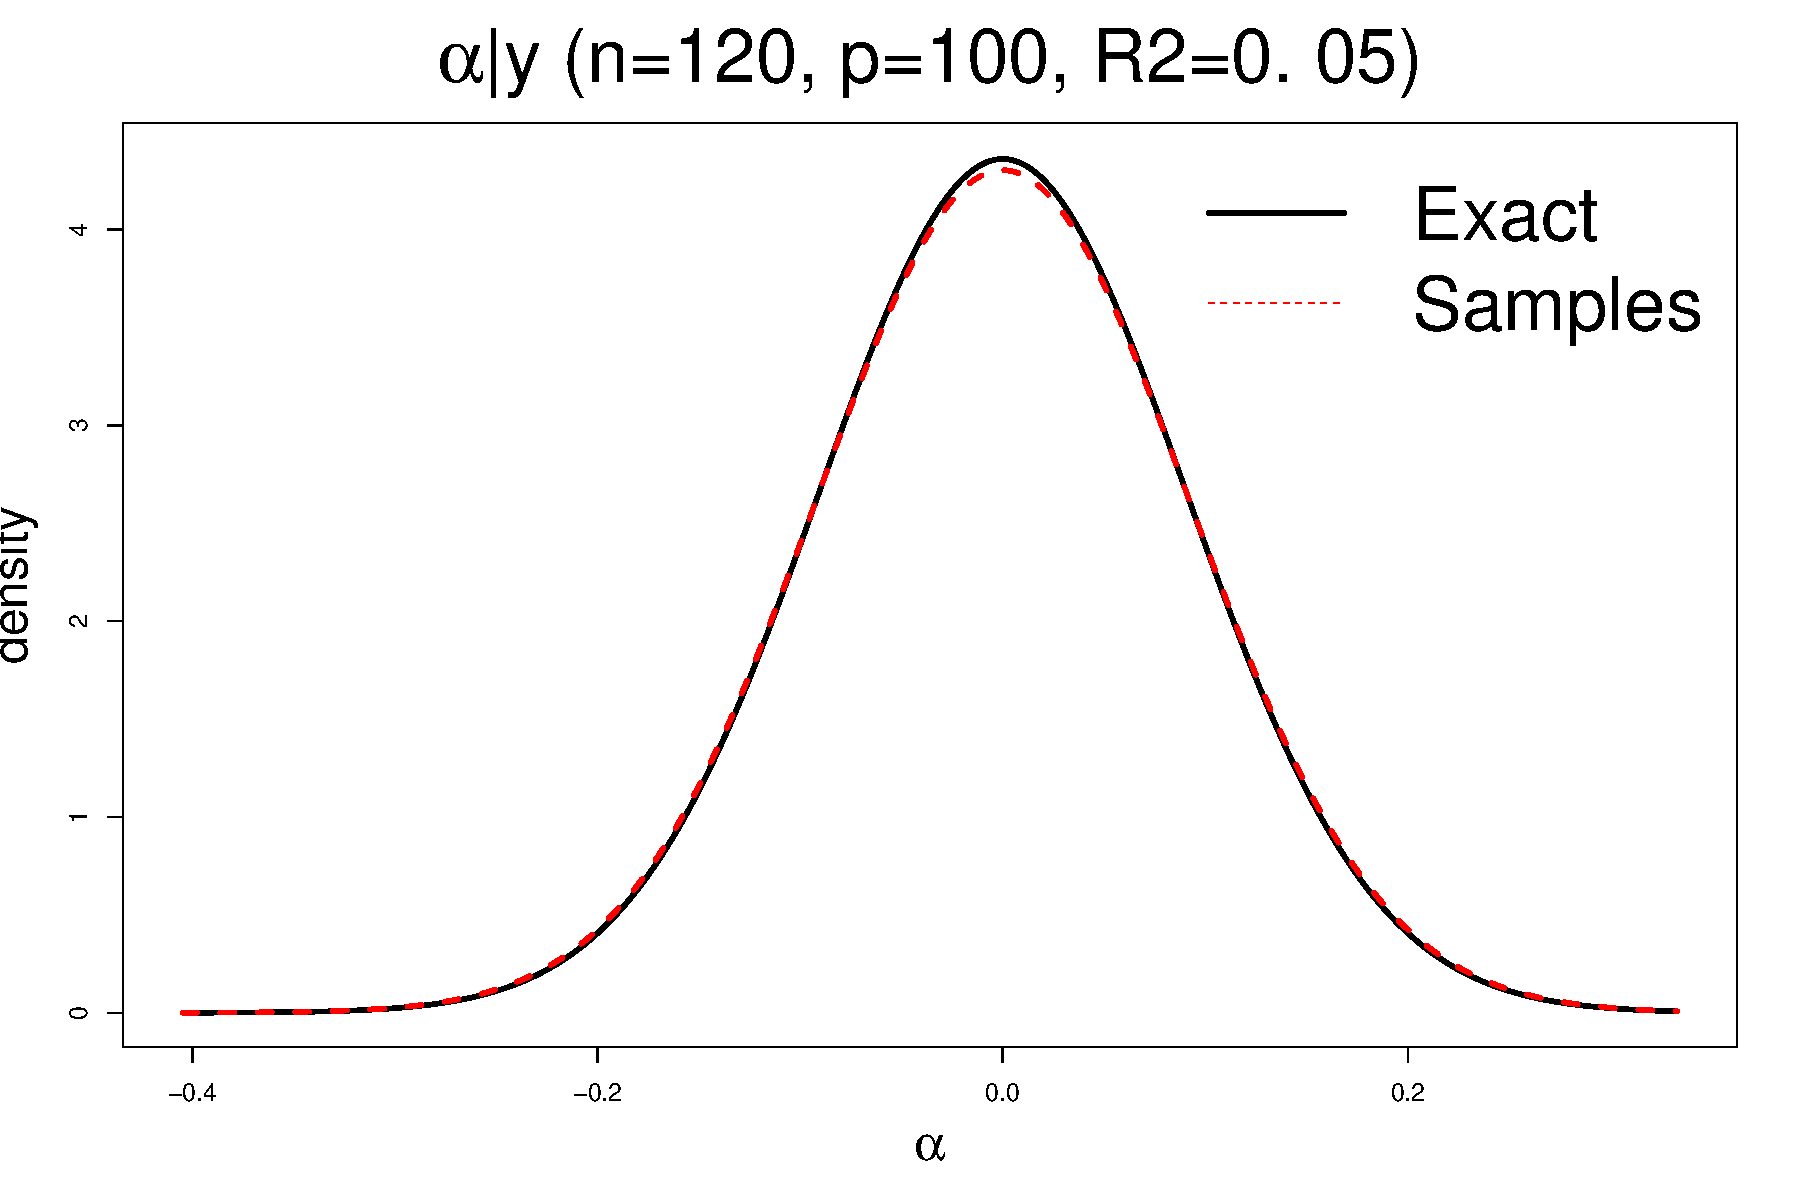
\includegraphics[scale=0.5]{code/alphaGivenY.pdf}
	\label{fig:alphaGivenY}
	\caption{The distribution of $\alpha | y$ for $n = 120$, $p = 3$, $20$ or $100$ and $R^2 = 0.05$ or $0.95$.}
\end{figure}

\begin{figure}
	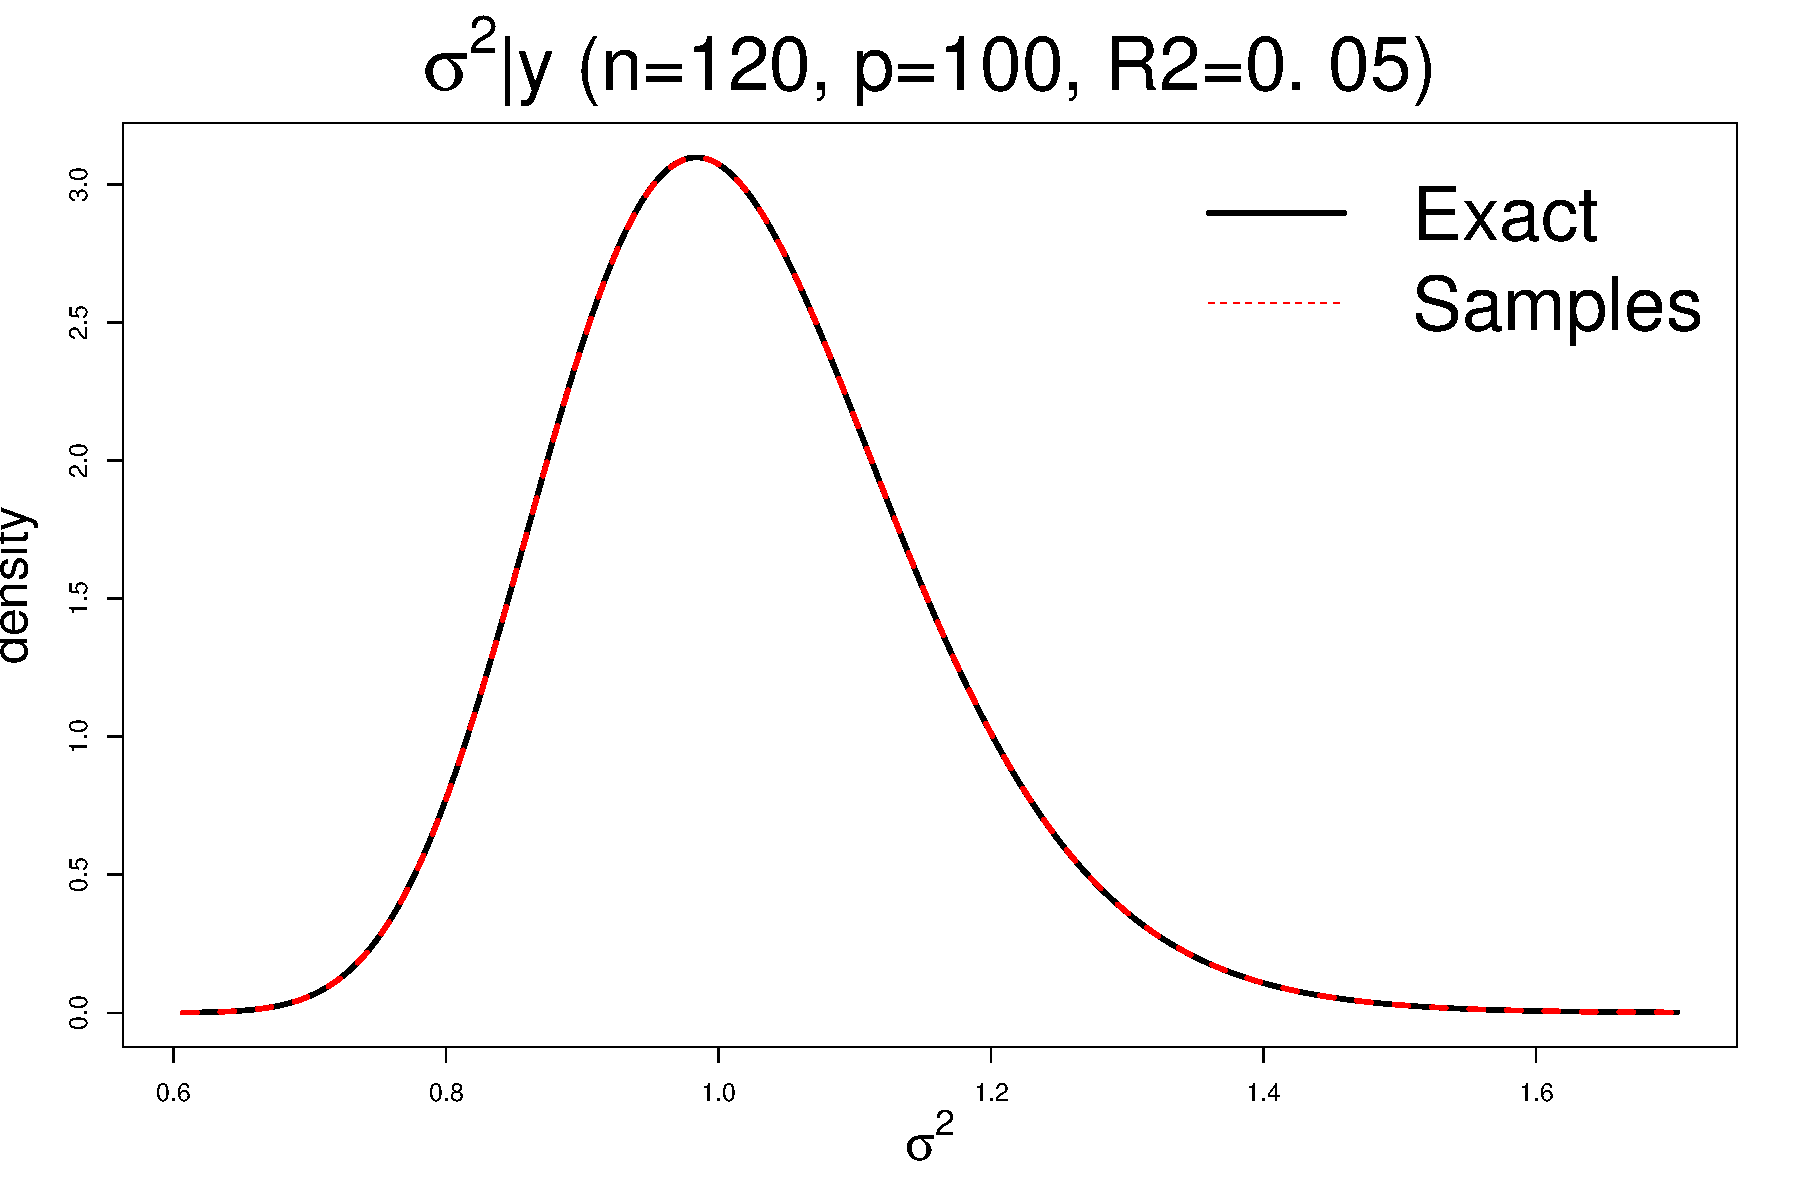
\includegraphics[scale=0.5]{code/sigma2GivenY.pdf}
	\label{fig:sigma2GivenY}
	\caption{The distribution of $\sigma^2 | y$ for $n = 120$, $p = 3$, $20$ or $100$ and $R^2 = 0.05$ or $0.95$.}
\end{figure}

\begin{figure}
	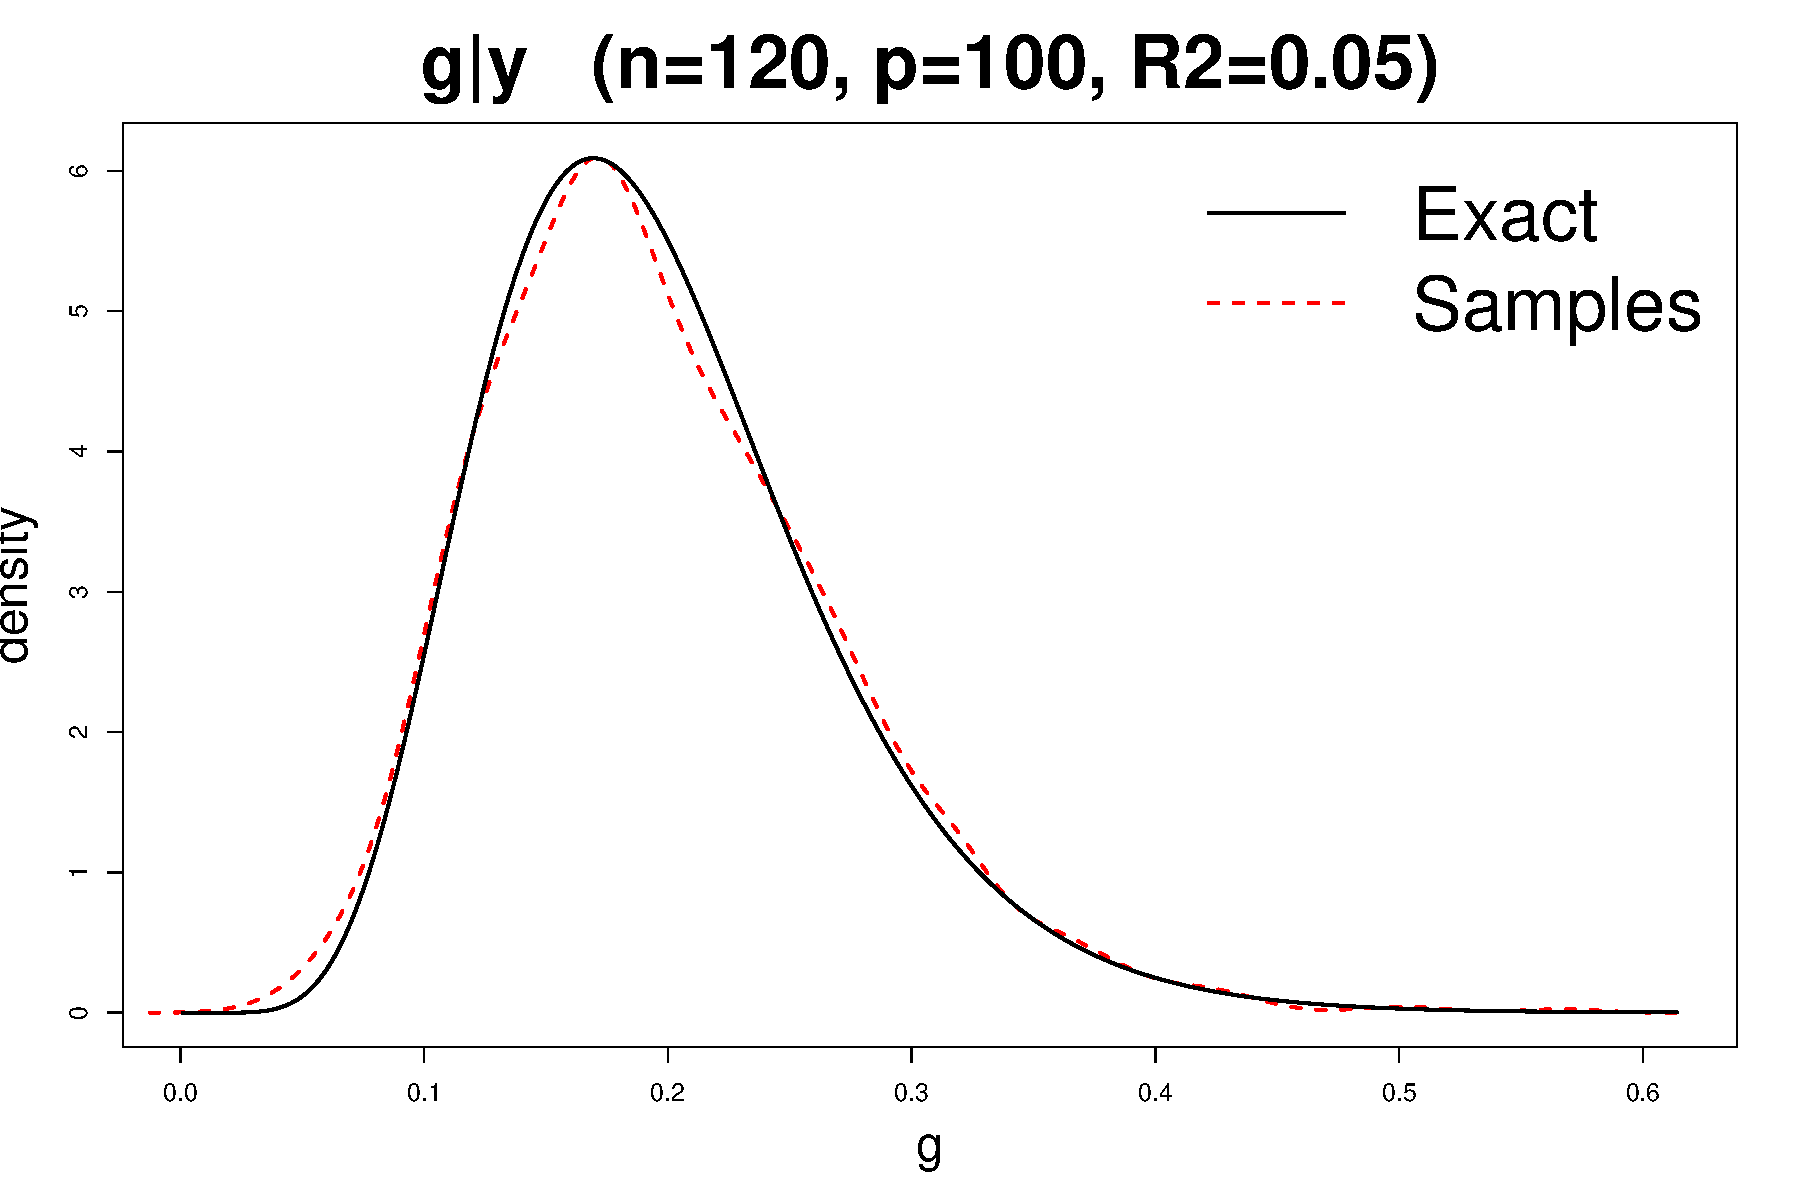
\includegraphics[scale=0.5]{code/gGivenY.pdf}
	\label{fig:gGivenY}
	\caption{The distribution of $g | y$ for $n = 120$, $p = 3$, $20$ or $100$ and $R^2 = 0.05$ or $0.95$,
					 when the prior on $g$ is the Beta Prime prior from \citep{Maruyama2011}.}
\end{figure}

\begin{figure}
	\includegraphics[scale=0.5]{code/BetaHitters.pdf}
	\label{fig:BetaHitters}
	\caption{The distribution of the regression co-efficient posteriors for the Hitters data set.}
\end{figure}


\subsection{Implementation details}
\label{sec:implementation}

We traverse the models in $\Gamma$ in Graycode order.
This ensures that as the algorithm moves from one model to another, only one covariate either enters or leaves
the model.
This allows us to use Rank-1 updates and downdates of $(\mX^\top \mX)^{-1}$ to greatly decrease the
computational cost of calculating $R_\vgamma^2$ from $\BigO(np^3)$ to $\BigO(np^2)$.
Special care was taken to minimise memory allocation and deallocation.
The \texttt{Rcpp} and \texttt{RcppEigen} libraries were used to ensure the implementation was performant.

Initially, $\vgamma = (1, 0, 0, \ldots, 0, 0)^\top$. So $(\mX_\vgamma^\top \mX_\vgamma)^{-1} =
(\vx_\vgamma^\top \vx_\vgamma)^{-1}$ which is a scalar, and so can be computed in $\BigO(n)$. Then the set of
possible models $\vgamma$ is iterated through in graycode order. This ensures that only one entry of $\vgamma$
changes as each model is visited, allowing the new $(\mX_\vgamma^\top \mX_\vgamma)^{-1}$ to be calculated
using the previous $(\mX_\vgamma^\top \mX_\vgamma)^{-1}$ and a rank-1 update. This allows us to avoid directly
computing the new $\mX_\vgamma^\top \mX_\vgamma$ and then performing a full inversion, reducing a $\BigO(n
p^3)$ operation to $\BigO(n p^2)$.

\mgc{Think about distribution of bit strings. What is the expectation of $p$? I think it's simply $p/2$}

\section{Conclusion and Discussion}
\label{sec:conclusion}

% This is all invalid now
The Variational Bayes approximation produces results which are almost identical to the exact likelihood.
The VB metholodology extends naturally to new situations, such as robust model fitting, mixed effects, missing
data, measurement error and splines. We are able to retain high accuracy with less computational overhead than
exact or MCMC.

All of the variational parameters in Algorithm \ref{alg:algorithm_two} except $\tau_g$ depend only on
$\tau_g$ and the fixed quantities $n$, $p$, $R^2$, $\mX$ and $\vy$. This allows us to optimise $\tau_g$
only, and then set the rest of the variational parameters at the end of the algorithm. The fact that only
univariate optimisation is required reduces the computation required to fit our approximation considerably,
which makes this algorithm applicable when speed and/or the ability to parallelise the algorithm are
paramount, such as model selection via structured Variational Bayes.

\appendix
\subsection{Useful Results}	

We first present the following results which will aid us in deriving the expressions required for fully Bayesian
inference over the parameters in the model.

\begin{equation}\label{res:01}
	\int \exp\left\{ -\tfrac{1}{2}\vx^T\mA\vx + \vb^T\vx \right\} d \vx = |2\pi\mSigma|^{1/2} \exp\left\{ \tfrac{1}{2}\vmu^T\mSigma^{-1}\vmu \right\}
\end{equation}
where $\vmu = \mA^{-1}\vb$ and $\mSigma = \mA^{-1}$.
 
If $\vone^T\vy=0$ the $R$-squared statistic can be expressed
\begin{equation} \label{res:02}
	R^2 = \frac{\vy^T\mX(\mX^T\mX)^{-1}\mX^T\vy}{\|\vy\|^2}
\end{equation}
where $R^2$ is the usual $R$-squared statistic associated with least squares regression.

Equation 3.194 (iii) of \citep{Gradshteyn1988} is
\begin{equation}\label{res:03}
	\int_0^\infty \frac{ x^{\mu - 1} }{(1 + \beta x)^\nu} dx = \beta^{-\mu} \mbox{Beta}(\mu,\nu - \mu) \quad \quad \mbox{(assuming $\mu,\nu>0$ and $\nu>\mu$).}
\end{equation}

Equation 3.385 of \citep{Gradshteyn1988} is
\begin{equation} \label{res:04}
	\int_{0}^1 x^{\nu - 1} (1 - x)^{\lambda - 1}(1 - \beta x)^{\varrho} e^{-\mu x} dx = \mbox{Beta}(\nu,\lambda) \Phi_1(\nu,\varrho,\lambda+\nu,-\mu,\beta)
\end{equation}

\noindent provided $\mbox{Re}(\lambda)>0$, $\mbox{Re}(\nu)>0$ and $|\mbox{arg}(1-\beta)|<\pi$.

